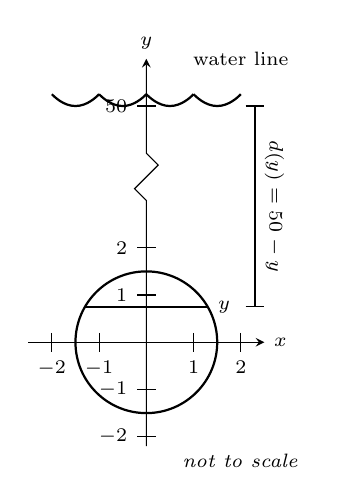
\begin{tikzpicture}[x=.6cm,y=.6cm,>=stealth]

\draw[thick] (0,0) circle (1.5);
										
\draw [{\colortwo},thick]  (-1.3,.75) -- (1.3,.75) node [right,black] {\scriptsize $y$};
										
\draw [->] (0,-2.2) -- (0,3)--(-.25,3.25) -- (0,3.5) -- (.25,3.75) -- (0,4) --(0,6) node [above] {\scriptsize $y$};
\draw [->] (-2.5,0) -- (2.5,0) node [right] {\scriptsize $x$};

\foreach \x in {-2,-1,1,2}
{
	\draw (\x,0.2) -- (\x,-.2) node [below] {\scriptsize $\x$};
}

\foreach \x in {-2,-1,1,2}
{
	\draw (.2,{\x}) -- (-.2,{\x}) node [left] {\scriptsize $\x$};
}

\draw (.2,5) -- (-.2,5) node [left] {\scriptsize $50$};

\foreach \x in {-1.5,-0.5,0.5,1.5}
{%
		\begin{scope}[shift={(\x*1,5)}]		
		\draw [{\colorone},thick] (-.5,.25) parabola bend (0,0) (.5,.25);
		\end{scope}
}
%
\draw (2,6) node {\scriptsize water line}
			(2,-2.5) node {\scriptsize \textit{not to scale}};

\draw (2.1,.75) -- (2.5,.75)
			(2.1,5) -- (2.5,5)
			(2.3,.75) -- node [pos=.5,rotate=-90,above] {\scriptsize $d(y) = 50-y$} (2.3,5);
			
\end{tikzpicture}


